\documentclass[tikz,border=2pt]{standalone}
\usepackage{amsmath}
\usepackage{pgfplots}
\pgfplotsset{compat=1.18}
\usetikzlibrary{arrows.meta}
\begin{document}
% Exercise 2.11: V1={-x1+2x2<=10, 3x1+x2<=10, x1-x2<=2} (corners (10/7,40/7), (3,1)) and
% V2={-x1+x2<=2, -2x1-x2<=-8, -x1-x2<=-5} (corners p=(2,4), (3,2)) meet only in p=(2,4);
% H={3x1+x2=10} separates them: V1 has the edge from (10/7,40/7) to (3,1) on H, V2 touches H only at p; normal a=(3,1).
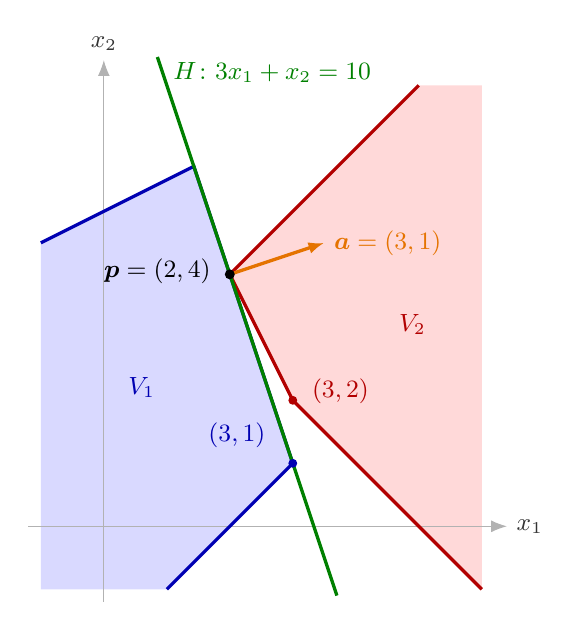
\begin{tikzpicture}[font=\small, >={Latex[length=2mm]}, x=0.8cm, y=0.8cm]
  % V1 and V2, clipped to the window
  \fill[blue!15] (-1,-1) -- (1,-1) -- (3,1) -- (10/7,40/7) -- (-1,4.5) -- cycle;
  \fill[red!15] (5,7) -- (2,4) -- (3,2) -- (6,-1) -- (6,7) -- cycle;
  % axes
  \draw[gray!60, ->] (-1.2,0) -- (6.4,0) node[anchor=west, gray!40!black] {$x_1$};
  \draw[gray!60, ->] (0,-1.2) -- (0,7.4) node[anchor=south, gray!40!black] {$x_2$};
  % boundaries
  \draw[blue!70!black, very thick] (1,-1) -- (3,1) -- (10/7,40/7) -- (-1,4.5);
  \draw[red!70!black, very thick] (5,7) -- (2,4) -- (3,2) -- (6,-1);
  % separating hyperplane H: 3x1+x2=10
  \draw[green!50!black, very thick] (0.85,7.45) -- (3.7,-1.1);
  \node[green!50!black, anchor=west] at (0.95,7.2) {$H\colon 3x_1+x_2=10$};
  % normal vector a=(3,1) at p
  \draw[orange!90!black, very thick, ->] (2,4) -- (3.5,4.5);
  \node[orange!90!black, anchor=west] at (3.5,4.5) {$\boldsymbol{a}=(3,1)$};
  % corners
  \fill[blue!70!black] (3,1) circle (1.6pt);
  \node[blue!70!black, anchor=south east] at (2.72,1.1) {$(3,1)$};
  \fill[red!70!black] (3,2) circle (1.6pt);
  \node[red!70!black, anchor=west] at (3.15,2.15) {$(3,2)$};
  % common point p
  \fill[black] (2,4) circle (1.8pt);
  \node[anchor=east] at (1.85,4.05) {$\boldsymbol{p}=(2,4)$};
  % set labels
  \node[blue!70!black] at (0.6,2.2) {$V_1$};
  \node[red!70!black] at (4.9,3.2) {$V_2$};
\end{tikzpicture}
\end{document}
